%&pdflatex

\documentclass[12pt]{report}

\usepackage{algorithm}
\usepackage{algpseudocode}
\usepackage{amsmath} % for implementation of the matrix environment
\usepackage{blindtext}
\usepackage{outlines}
\usepackage{caption}
\usepackage[utf8]{inputenc}
\usepackage{color}
\usepackage[pdftex]{graphicx} \graphicspath{{./plots/}}
\usepackage{epstopdf} \epstopdfsetup{update} % only regenerate pdf files when eps file is newer
\usepackage{float} % figure groups aka floats
\usepackage{forest} % for MFS elimination tree diagram
\usepackage[left=3.5cm, right=2.5cm, bottom= 3cm]{geometry} % margins
\usepackage[shellescape,latex]{gmp} % metapost for UMLs
\usepackage[hidelinks]{hyperref} % ToC/LoA/LoF/LoT entries are links
\usepackage{mathptmx} % Times New Roman like font
\usepackage{array}
\usepackage{titlesec}
\usepackage{comment}
\usepackage{pdfpages} % for inserting pdf as the initial pages
\usepackage{setspace} \onehalfspacing % 1.5 line spacing
%\usepackage{subcaption}
\usepackage{xfrac} % nice slanted fractions
\usepackage{graphicx}
\usepackage[english]{babel}
\usepackage[utf8]{inputenc}
\usepackage{fancyhdr}
\usepackage{subfig}

\pagestyle{fancy}
\fancyhf{}

\captionsetup[figure]{labelfont={bf}, textfont={small}}
\captionsetup[subfigure]{labelfont={bf}, textfont={small}}

\newcommand{\bt}{\blindtext}
\newcommand{\eps}{\varepsilon}
%\newcommand{\rev}[1]{\textcolor{red}{#1}}
\newcommand{\rev}[1]{#1}
\newcommand{\T}[1]{\texttt{#1}}
\newcolumntype{P}[1]{>{\centering\arraybackslash}p{#1}}

\algnewcommand\And{\,\textbf{and}\,}
\algnewcommand\Or{\,\textbf{or}\,}
\algnewcommand{\LineComment}[1]{\State \(\triangleright\) #1}
\usepackage[english]{babel}

\titleformat{\chapter}[display]
{\normalfont\bfseries}{}{0pt}{\Huge}

\begin{document}


\includepdf[pages={-,{}}]{initial-pages.pdf} % `-' for all pages, `{}' for an empty page

\tableofcontents
%\chead{Learning strategies in multi agent system}
%\cfoot{Jakub Boliglowa - Computer Science}
\fancyhead[LE,LO]{\leftmark}
%\fancyhead[RE,RO]{\rightmark}
\fancyfoot[LE,CO]{Learning strategies in multi agent system}
\fancyfoot[LE,RO]{\thepage}

\renewcommand{\headrulewidth}{1pt}
\renewcommand{\footrulewidth}{1pt}
\chapter{Introduction}


\quad Nowadays, research and development of artificial intelligence has become widespread in every field of science. The emerging trend of completely replacing man with a machine poses new challenges to create a human-like being in the context of decision-making skills. The human ability to perceive the world (the environment in which it operates) and the ability to learn is a major challenge when trying to create beings similar to humans. 
Joint decision-making might be better than in the case of a decision by a single individual. A system as a structure composed of agents who have the ability to solve tasks based on decision-making. In this work, various approaches to agent learning process will be considered to create final prediction. By appointing agents-experts in a given field by modifying their attributes of which they perceive the environment, there is a chance to get a better prediction model.

In the bibliography, there will be modern state-of-the-art papers described multi-agent systems, artificial intelligence used in these types of systems and some most important milestones of this field of knowledge as well as some psychological works about human behaviour.

\section{Goal of the thesis}


\quad The goal of this work is to research and analyze the strategies of learning in agent systems. After analyzing actual solutions which are created over multi agent systems would be considered style of learning and perceving environemnt by each agent.
In these work will be used advanced ensemble learning techniques. Different types of approaches will be used to construct the final prediction model. What differentiates this work from other projects, is mainly the approach to learning for each agent. An environmental overhead that limits the perception of agents, making them specific experts in a given field
As part of the work will be the creation of simulation groups having human traits whose task will be to take the best decision. Strategies of using agents in service are discussed, in relation to the imposed conditions by the system environment. The creation of the model by the agent with limited ability to perceive the environment will be checked for many combinations of available machine learning algorithms. What's more, combining these models, including those that proved to be relatively inferior, will improve the final predictive model.
Finally, the problem under consideration will be a set of data determining the prices of plots (including houses) in the USA based on parameters determining: geographical location, size of the property, condition and construction of the house.

\section{Elo}

\quad siema elo
co tam


\chapter{Machine learning in multi agent system} 
\label{chap:Machine learning in multi agent system}

In this chapter, it will be presented an overview of the state of the art in the areas related to the topic of this work. In first subsection is a description of several types of machine learning used in agent systems. Learning process of agent is also demonstrated. Various machine learning approaches (supervised, semi-supervised, unsupervised, reinforcement) were quoted together with the methods and results of learning by agents.

Next subsection in this chapter has been devoted to the explanation of ensemble learning. State of the art of this thesis is focused on: stacking, boosting, bagging techniques. The application of these methods and important conclusions that were formulated during the experiments were quoted.

Then, in following subsection there is a definition of regression and classification algorithms. Focused mainly on: Decision Tree, Support Vector Regressor, K nearest neighbours, Bayesian Ridge. The literature review includes the use of these methods in agent systems and the justification for their use in solving the current problem.

Another subsection is dedicated to the presentment of prepared multi agent system. The architecture of the following system is estabilished, along with a details of created environment. Roles and types of existing agents are exposed. Relations between agents are shown. The way of perceiving the environment (sensors) and the possible interactions are documented. 

\newpage
\section{Types of machine learning}

Nowadays, the subject of data science has evolved that four types of machine learning approaches has been distinguished. Research on artificial intelligence arose from analyzing the behavior of the human brain. Main difference based on the type of data they input and output and the type of task or problem that they are intended to solve. Thus, machine learning algorithms are organized into taxonomy, based on desired outcome of the algorithm. 
Defined approaches organized in the following groups  \cite{TypesOfMachineLearning}:
\begin{outline}[]
	\1 Supervised learning --- where the algorithm maps incoming data (input) to desired output,
	\1 Unsupervised learning --- this approach models a set of inputs (unavailability of labeled examples),
	\1 Semi-supervised learning --- labeled and unlabeled examples ad combined in order of creation an appropriate function or classifier,
	\1 Reinforcement learning --- where algorithm is trained using a system of reward and punishment. Every action has impact in the environment that generates a feedback that guides the learning method.
\end{outline}

The variety of tasks that are solved by artificial intelligence forces a broader view of the issue under consideration. The essence of this is the proper selection of existing methods of artificial intelligence in order for the model created to be the best.  


\begin{center}
	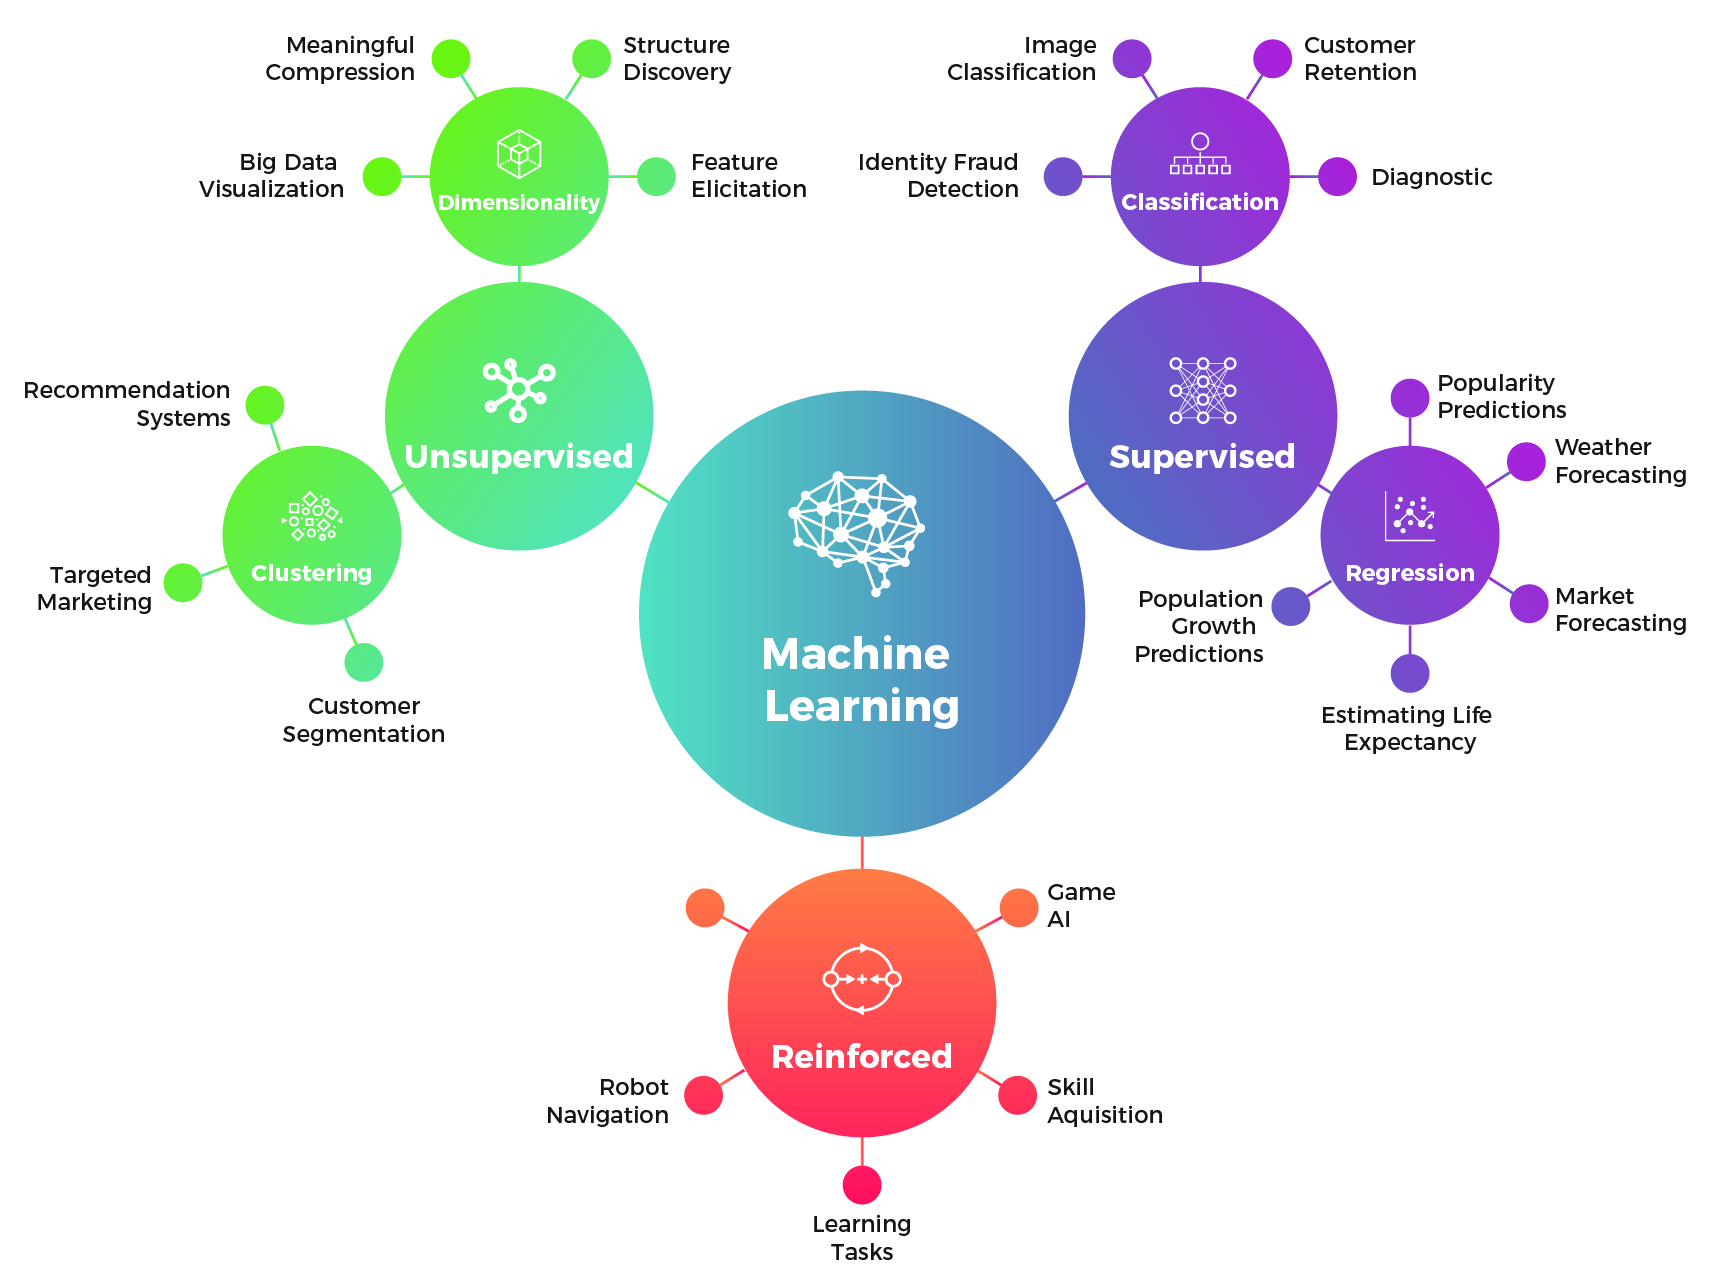
\includegraphics[width=1\textwidth, keepaspectratio]{diagrams/machine_learning_model.png}
	\center
	\captionof{figure}{The application of artificial intelligence along with the division of machine learning into these branches \cite{MachineLearningModels}.} 
	\label{fig:MachineLearningTypes}
\end{center}

On Figure ~\ref{fig:MachineLearningTypes} are shown examples of different approaches of using artificial intelligence. Machine learning algorithms have found wide application in scientific world. 
Applying artificial intelligence in systems has been popular recently. Nowadays, collecting data takes place everywhere. In this way, the information collected can be used to solve and support decision-making process. Along with the development of issues related to the subject of AI, many extensions of classic machine learning methods have been created.
The technique chosen for the solution depends on the type of data and is  often supported by another learning method. However, the use of machine learning does not always bring the intended results. This is done, e.g by the lack of adequate data (insufficient quality or quantity), so there is a need to use other methods known to date.


\subsubsection{Supervised learning}
Supervised learning is a learning model built to make prediction with a given an unforeseen input instance. Known input data set and its mapped output values are taken to learn (training process) the regression or classification model. Therefore, classification and regression algorithms are used to develop predictive model which describes a given issue. Thus, the model is predictive because it relies on statistical and probabilistic techniques to predict the correct mapping values based on historical observations \cite{SupervisedUnsupervised1, SupervisedLearning}.

\begin{figure}[H]%
	\centering
	\subfloat[Linear regression]{{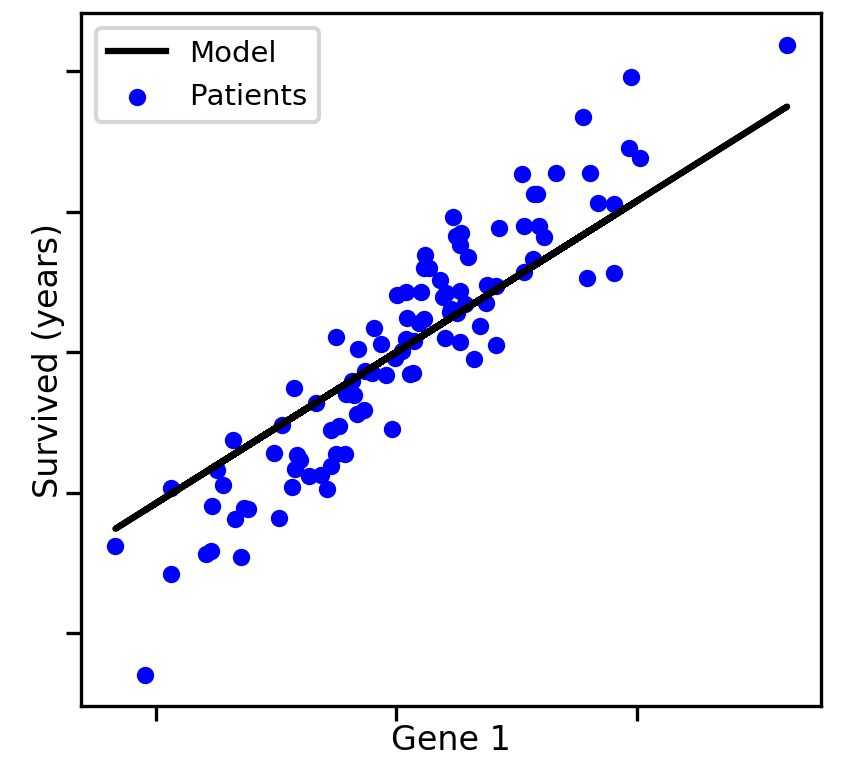
\includegraphics[width=5cm]{diagrams/supervised_regression_patients} }}%
	\qquad
	\subfloat[Object classification]{{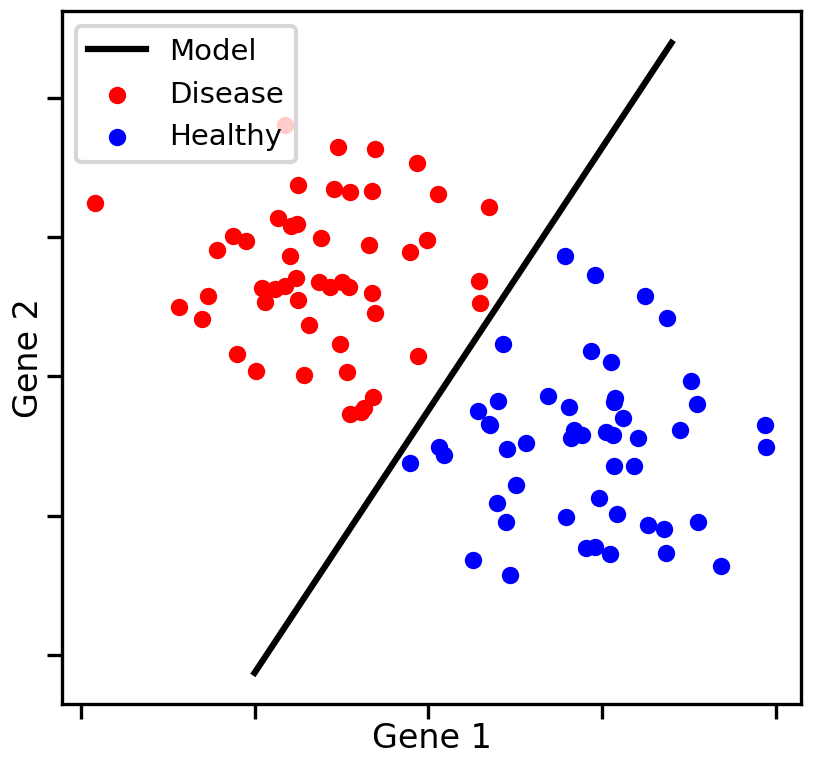
\includegraphics[width=5cm]{diagrams/supervised_classification_patients} }}%
	\caption{Regression and classification as a supervised technique. Epidemic spread by distinguishing between smaller sub-tasks \cite{ClassificationAndRegression}.}%
	\label{fig:SupervisedLearningFigure}%
\end{figure}

Mostly depends on problem category which needs to be solved supervised learning provides various techniques of creating predictive model \cite{RegressionInML, ClassificationSupervisedLearning}:
\begin{enumerate}
	\item Regression techniques --- predict or forecast continuous responses. The goal is to estimate the correct output, given a feature vector. There are several types of regression concepts: simple linear regression (presented on figure  \ref{fig:SupervisedLearningFigure}), polynomial regression, support vector regression, decision tree regression, random forest regression
	\item Classification techniques (example is presented on figure  \ref{fig:SupervisedLearningFigure})--- the goal is to predict the categorical class labels (discrete, unordered values, group membership etc.) of new instances based on past observations. There are two main types of classification problem: binary classification and multi-class classification.
\end{enumerate}



In \cite{SLKhaled}, Khaled and other authors noticed that applying various supervised machine learning algorithms to the problem is not easy because there is a possibility to provide "correct" behavior for a given decision situation. In this paper, there is a consideration above multi-agent learning aspects. Furthermore, based on Weiss \cite{Weiss} publication they described aspects for characterizing learning in multi agent system:
\begin{enumerate}
	\item degree of decentralization --- learning centralized or decentralized,
	\item interaction-specific aspects (by Weiss \cite{Weiss} "level of interaction") --- nature of interactions,
	\item involvement specific aspects --- global or local learning,
	\item goal-specific aspects --- selfish or collective agent goals
\end{enumerate} 

As a consequence, they created comparison of supervised learners an the learning aspects based on other related works. Fish bank game is solved by Sniezynski \cite{Sniezynski2009SupervisedRL} using supervised rule learning. Enhance coordination in environment of heterogeneous agents are done using learning coordinated procedures by Garland and Alterman \cite{Garland2004AutonomousAT}. Learn individual's ontoligies in the field of semantic webs using inductive learning algorithms was under consideration by Williams \cite{Williams2004LearningTS}. Gehrke and Wojtusiak contemplated at route planning using rule induction algorithm \cite{Wojtusiak}. Decision tree learning was used to support plan applicability testing, through adding learning capabilities into BDI model by Airiau et. al \cite{Airaiu}. 
Hence the conclusion about supervised learners and learning aspects are formulated in presented table.

\begin{table}[H]
	\centering
	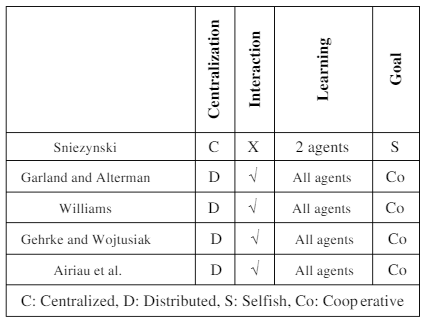
\includegraphics[width=7cm, keepaspectratio]{diagrams/related_work/Supervised_learners_vs_learning_aspects}
	\center
	\captionof{figure}{Supervised learners vs learning aspects \cite{SLKhaled}.} 
	\label{tab:LearningAspects}
\end{table}


In \cite{SLSardinha2004EngineeringML}, Sardinha, Choren, Milidiu and Pereira de Lucena proposed a methodology for introducing machine intelligence in multi-agent system. As a case study is presented Trading Agent Competition. They implemented methodology which reduces the complexity of modeling, implementing and evaluating learning techniques in large scale multi agent-system. This approach provides an improvement of perfmormance about 98\% due to the introdution of supervised machine learning algorithms. 




\subsubsection{Semi-supervised learning}

Semi-supervised learning is used to perform certain learning tasks using labeled and unlabeled data  \cite{SemiSupervisedLearning1}. In fact, it permits harnessing the large amounts of unlabeled data which exists in many use cases in combination with typically smaller sets of labeled data - hence this learning approach is useful when the cost associated with labeling is too high to allow a fully labeled training process. Therefore it can be used with methods such a classification, regression and prediction. 

\begin{center}
	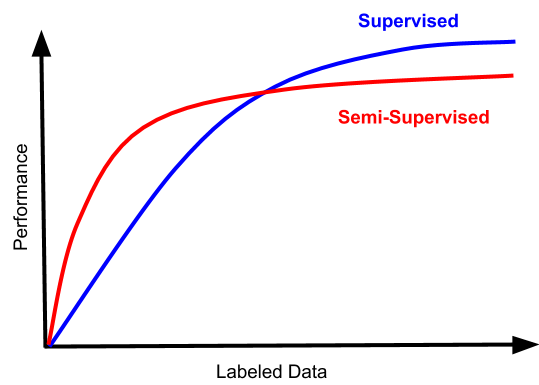
\includegraphics[width=8cm, keepaspectratio]{diagrams/semi_supervised}
	\center
	\captionof{figure}{Training process performance  depends on size of labeled data on the example of blockchain data set \cite{SemiSupervisedLearning2}.} 
	\label{fig:SemiSupervisedLearning}
\end{center}

In paper \cite{SSPredicition}, authors have done research on analyzation and predicition human flow. They constructed a multi-agent system which simulate and generate prepared data of people flows around a large facility. Different approach to learning (deep learning) were benchmarked. Simulation data and real data were used in the learning phase, so learning can be considered as semi-supervised learning. 

\subsubsection{Unsupervised learning}

Unsupervised learning is completely different approach than it was described in previous subsections. Most or all of the data cannot be presorted or preclassified beforehand, so the complexity of machine learning algorithm is growing dramatically causing the process more and more time intensive. 
However, this makes unsupervised learning seductive in applications where data is cheap to obtain, but labels are either expensive or not available. The main assumption of the approach is to discover the structure through common elements in data.
Popular techniques include clustering and dimensionality reduction
\cite{UnsupervisedLearning1, UnsupervisedLearning2}.

\begin{figure}[H]%
	\centering
	\subfloat[Supervised learning \cite{PolynomialRegression}]{{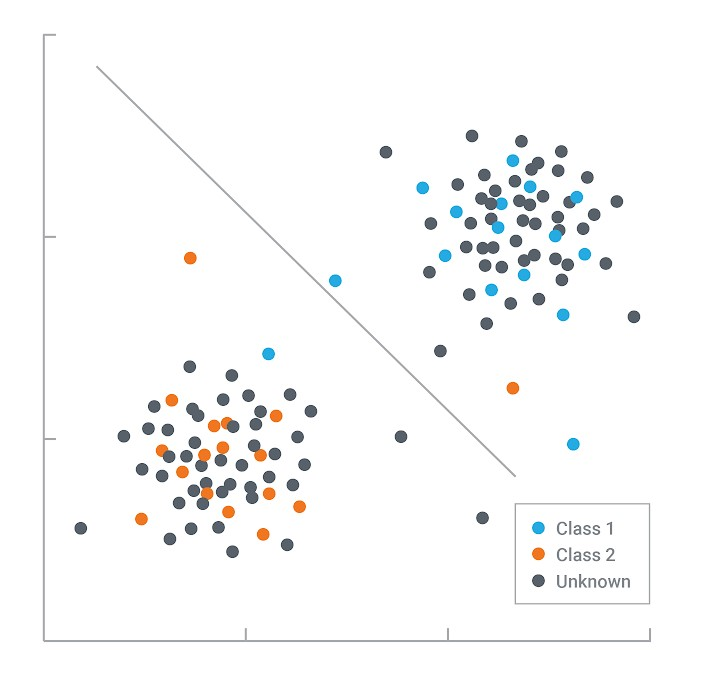
\includegraphics[width=5cm]{diagrams/supervised_diagram} }}%
	\qquad
	\subfloat[Unsupervised learning \cite{SupervisedUnsupervised1}]{{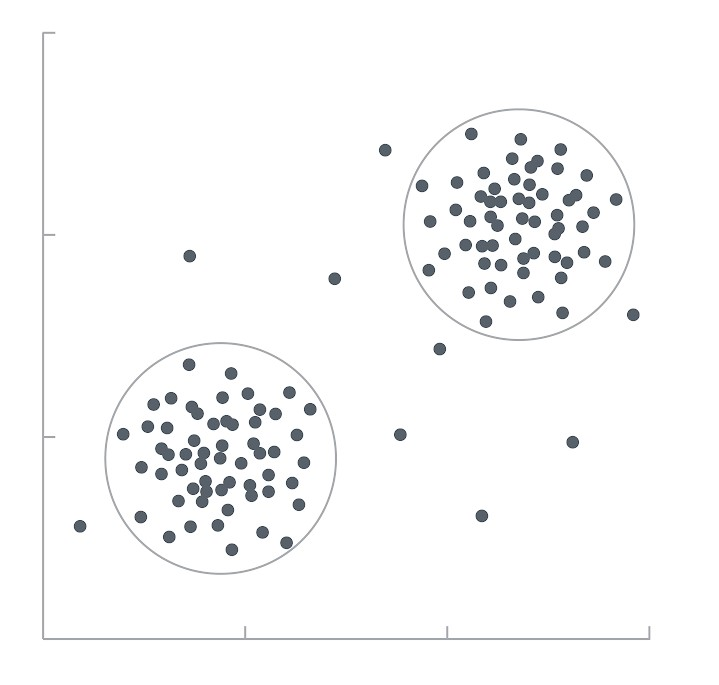
\includegraphics[width=5cm]{diagrams/unsupervised_diagram}}}%
	\caption{Differences in approach to learning on the example of classification objects.}%
	\label{fig:DifferencesLearning}%
\end{figure}

In \cite{Duarte2015MPDraughtsUL}, authors proposed usage of unsupervised learning injected into multi-agent system for Checkers game whose architecture is based on adaptive and multi-layer perception neural network. Besides there are several types of agents so the agents are trained for a distinct stages of the game. Each agent corresponds to a multi-layer perception neural network whose weights are updated by Temporal Difference methods \cite{TemporalDifferenceLearning}.

\begin{center}
	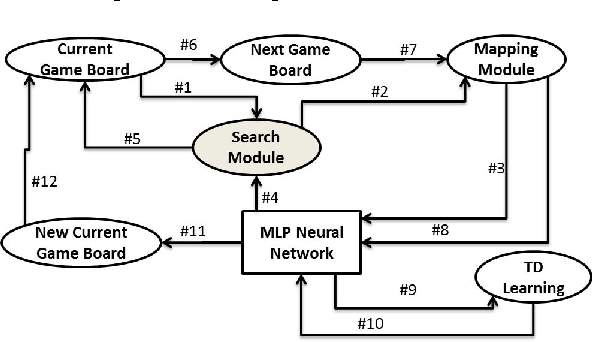
\includegraphics[width=8cm, keepaspectratio]{diagrams/related_work/ULCheckers}
	\center
	\captionof{figure}{Learning process for each agent \cite{Duarte2015MPDraughtsUL}.}
	\label{fig:ULChekersLearningProces}
\end{center}

In fact, at the late game each agent is an expert in a particular profile (have been trained to become an expert) of endgame board-state. On the figure \ref{fig:ULChekersLearningProces} is presented learning process for each agent.
As a conclusion: creating environment where agents have a chance to become an expert could have positive influence on working entire system and using an adaptive neural network improve overall performance of the multi-agent system.

\subsubsection{Reinforcement learning}
This learning approach has three primary components: the agent (the learner or actor), the environment (everything the agent interacts with) and actions (how agent interact). Reinforcement learning is concerned about an agent that interacts with the environment and learns an optimal policy by trail and error \cite{ReinforcementLearning2}.  Feedback loop based on which the agent is rewarded is shown on figure \ref{fig:ReinforcementLearning}. The reward received is defined by the \emph{reward function}, which maps state/action pairs to the real number \cite{ReinforcementLearning1}. The objective is for the agent to choose actions that maximize the expected reward over a given amount of time.

\begin{center}
	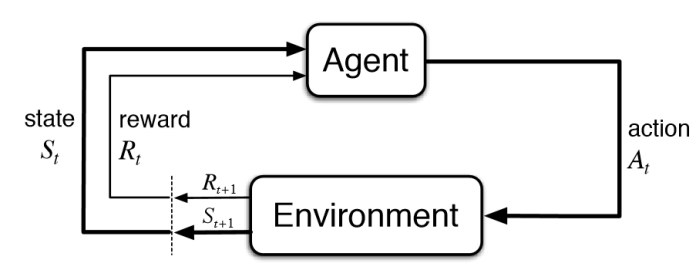
\includegraphics[width=9cm, keepaspectratio]{diagrams/reinforcement_learning}
	\center
	\captionof{figure}{Basic idea and elements involved in a reinforcement learning model \cite{ReinforcementLearning2}.} 
	\label{fig:ReinforcementLearning}
\end{center}
In \cite{RLRealtedWorkShops}, Deepak and Kulkarni proposed a novel approach to multi-agent cooperation for dynamic product availability in the market. Agents cooperate with each other to improve possible profits, thus it is said that retailers learn cooperatively depends on the actual situation. The problem turns out to be Markov decision process model because of the dealer's inventory strategy, refill period and entry procedure of the customers. 

Cooperation methods of cooperative reinforcement
learning of each agent have been proposed:
\begin{enumerate}
	\item group method --- rewards are distributed in a sequence of steps,
	\item dynamic method --- for each action rewards are distributed, 
	\item goal-oriented method --- when the agent achieve the goal-state then follows reward distribution. 
\end{enumerate}

\begin{center}
	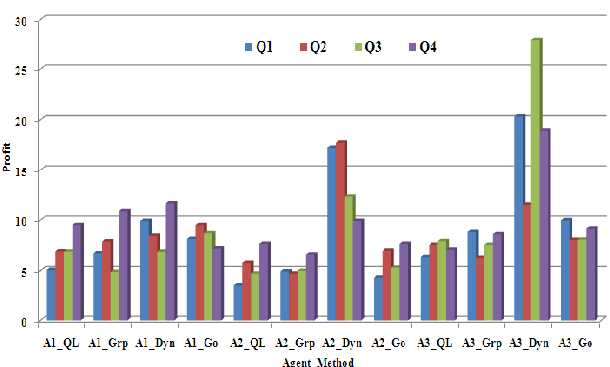
\includegraphics[width=10cm, keepaspectratio]{diagrams/related_work/RLprofit}
	\center
	\captionof{figure}{Quarterly profit earned by all sellers using four methods of learning \cite{RLRealtedWorkShops}.} 
	\label{fig:RLRelatedWork}
\end{center}

As a conclusion from the article, is that cooperation methods gives a healthy performance in high-density, incompletely and composite situation, thus methods are able to guarantee best rewards through learning process and change with a group in incomplete action strategies.

\newpage
\section{Ensemble learning}
Ensemble learning is a machine learning paradigm where multiple learners are trained to create base model \cite{Zhou2009}. Ensemble learning attempts to construct a set of hypotheses and combine them to use, but in contrast to the classical approach of machine learning, in which learners in one case, they learn one hypothesis based on the training data. 
Applying ensemble methods can boost weak learners to strong learners. Weak learners are better than random guess but cannot make accurate and satisfactory predictions. According to the hypothesis that weaker learner will strengthen potenially more promising learners in the decision-making process.

Considering how to create base learners, ensemble methods can be divided into two groups:
\begin{enumerate} 
	\item sequential ensemble methods - base learners are generated sequentially,
	\item parallel ensemble methods - base learners are generated in parallel.
\end{enumerate}
There are common types of ensembles:
\begin{itemize}
	\item Bayes optimal classifier
	\item bootstrap aggregating (bagging)
	\item boosting
	\item Bayesian model averaging
	\item Bayesian model combination
	\item bucket of models
	\item stacking
\end{itemize}
\begin{comment}
## need citiation 
## https://link.springer.com/chapter/10.1007%2F978-3-642-12101-2_35
opiopiop
\end{comment}

In ensemble techniques, there are many taxonomies \cite{ComparisonBagging}. Under consideration is a group of methods based on data resampling. Consequently, one method from this group generates different training sets to obtain unique learner.

\begin{center}
	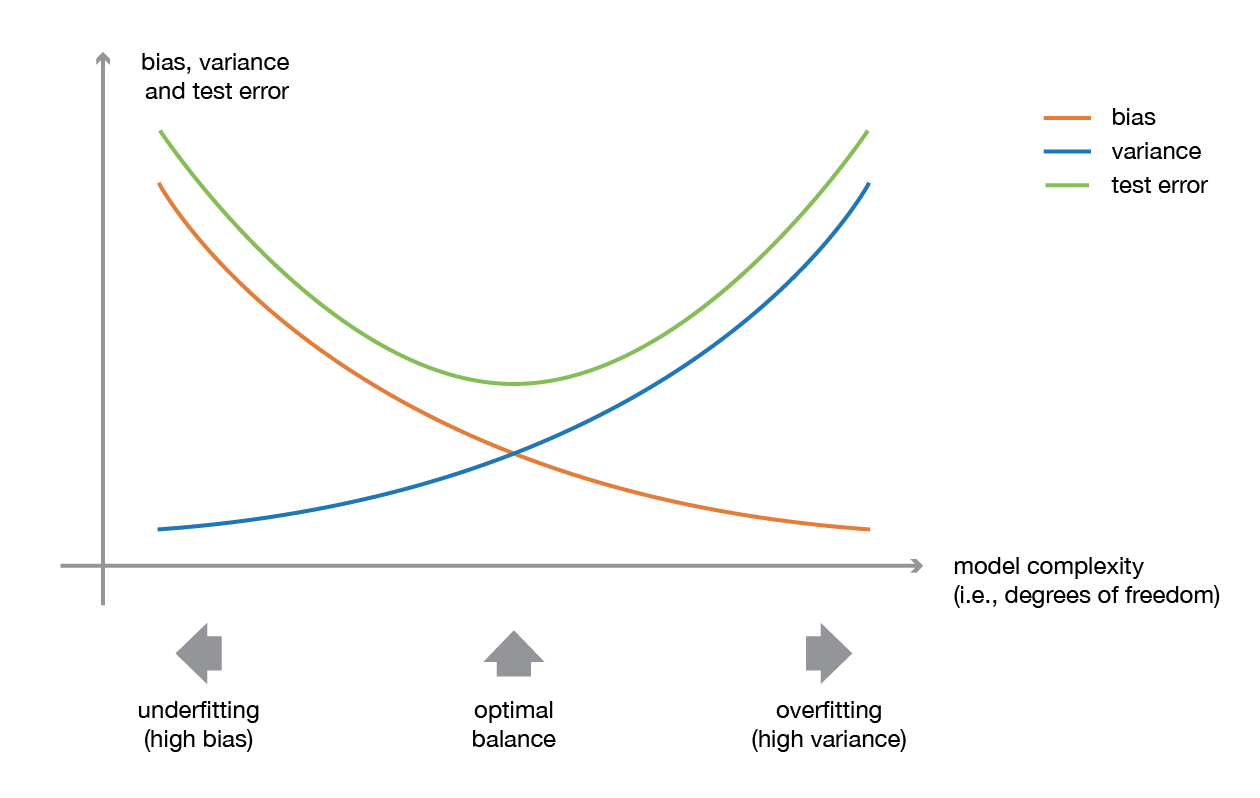
\includegraphics[width=10cm, keepaspectratio]{diagrams/tradeoff}
	\center
	\captionof{figure}{Bias-variance trade-off \cite{EnsembleMethodsTradeOff}.}
	\label{fig:EnsembleTradeOff}
\end{center}
Figure \ref{fig:EnsembleTradeOff}, demonstrate a trade-off between bias, variance, test error values and model complexity. In fact, the requirement to solve the problem using created model is to have enough flexibility to resolve the underlying complexity of the data, but also having not too much degrees of freedom to avoid high level of variance and be more robust.
Described techniques were mainly used as a meta-algorithms which combine several machine learning algorithms in order to decrease variance (bagging), decrease bias (boosting) and improve predictions (stacking).

\subsubsection{Stacking}
Stacking as a ensemble learning method is popular to achieve greater predictive accuracy using combination of lower level base learner (In fact it is one single high-level base learner created as a combination low-level learners) \cite{StackingDefinition}. Collecting the output of each base learner into a new set of data is a first step in this approach. Care is taken to ensure that the base learners are formed from a batch of training data. A new data is treated as a data for another learning problem.
\begin{center}
	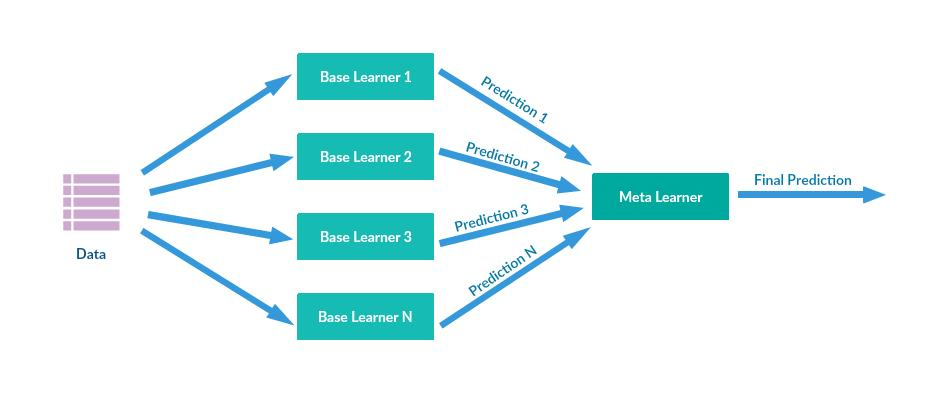
\includegraphics[width=12cm, keepaspectratio]{diagrams/stacking.jpg}
	\center
	\captionof{figure}{Meta learner as a combination of base learners  \cite{stackingEnsemble}.}
	\label{fig:Stacking}
\end{center}
In the fig. \ref{fig:Stacking} is shown data flow using stacking as an ensemble method. Different weak learners are fitted independently. However, using an extension of stacking is getting more and more popular. Modified version is called multi-level stacking, consists doing stacking with multiple layers.
\subsubsection{Bootstrap Aggregating (Bagging)}
Bagging is an ensemble method for improving unstable estimation or classification schemes. Considered method is about splitting training data into smaller constant parts. For a given training set of size \textit{s}, bagging draws \textit{t} random instances with replacement (i.e. using a uniform distribution) \cite{SupervisedMachineLearningReviewClassification, BaggingDef}. Building ensembles using bagging method based on different part of training data is done with learning by single method. 

In \cite{BreimanBagging}, Breiman defined bagging as a variance reduction technique for a given base procedure, mostly a decision trees or functions which fitting a linear model.
Breiman also considered about number of Bootstrap replicates. Several number of replicates where benchmarked for classification and regression, however number of enough replicates depends mainly on the data set(size and number of labels).
\begin{center}	
	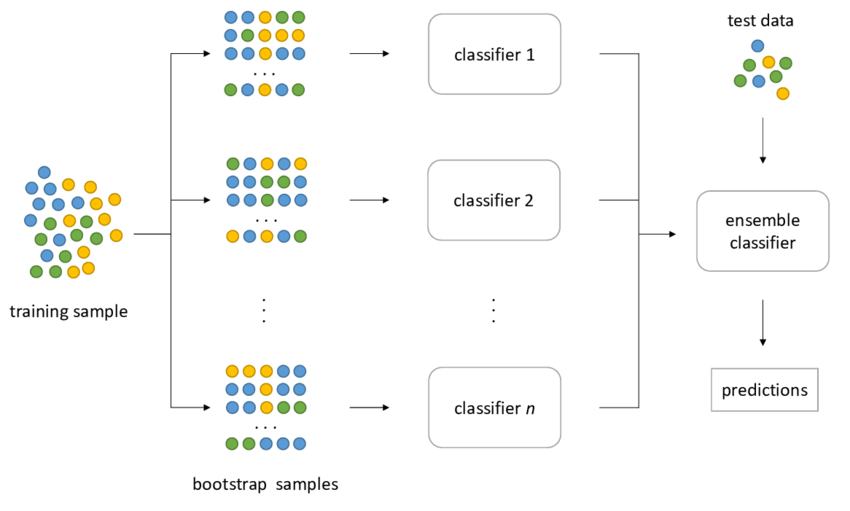
\includegraphics[width=12cm, keepaspectratio]{diagrams/bagging.png}
	\center
	\captionof{figure}{In bagging, training instances can be sampled several times for the same predictor \cite{baggingEnsemble}}
	\label{fig:Bagging}
\end{center}

Figure \ref{fig:Bagging} gives a sample how Bootstrap Aggregating works on a imaginary set of data. Breiman (1996) showed the effectiveness of using these ensemble method. Bagging is effective on "unstable" learning algorithms where making small changes have large influence on predictions. In fact, Breiman in 1996 claimed about unstable learning algorithms and nowadays neural networks and decision trees are simple examples of unstable learning algorithms. 

\begin{table}[H]
	\centering
	\captionof{table}{Bagged Misclassification rates. Results appeared for the 10, 25, 50, 100 numbers of bootstrap replicas used on waveform dataset \cite{BreimanBagging}.}
	\label{tab:BaggingReplicatesTable} 
	
	\begin{tabular}{|P{5cm}|P{5cm}|} \hline
		No. Bootstrap Replicates & Misclassification Rate \\ \hline
		10                       & 21.8                   \\ \hline
		25                       & 19.4                   \\ \hline
		50                       & 19.3                   \\ \hline
		100                      & 19.3                  \\ \hline
	\end{tabular}
\end{table}
In table \ref{tab:BaggingReplicatesTable} are shown the results of using bootstrap replicates and its misclassification rates. Breiman observed, that getting most of the improvement is using only 10 bootstrap replicates. The unbagged rate is 29.1. Consequently, it can be seen that the trade off between the efficiency and complexity of the learning algorithm and the profit in the form of a misclassification metric is when increasing the number of replicas we do not achieve much improvement. It is better to use less than 25 replicas on the used data set.

\subsubsection{Boosting}
Boosting keeps track of the performance of the learning algorithm and concentrates on instances that have not been correctly learned. This ensemble method also uses different subset of training data. Rather than random choosing the training instances using uniform distribution, this approach chooses the training subsets to favor the instances that have not been accurately learned \cite{SupervisedMachineLearningReviewClassification}. This approach considers homogenous weak learners and learns them sequentially in a very adaptative way to combines them following a deterministic strategy. In fact, after several steps, the predicition is done by taking a weighted vote of predictions of each classifier, with the weights which are proportional to each classifier's accuracy metric on its training set. 

\begin{center}
	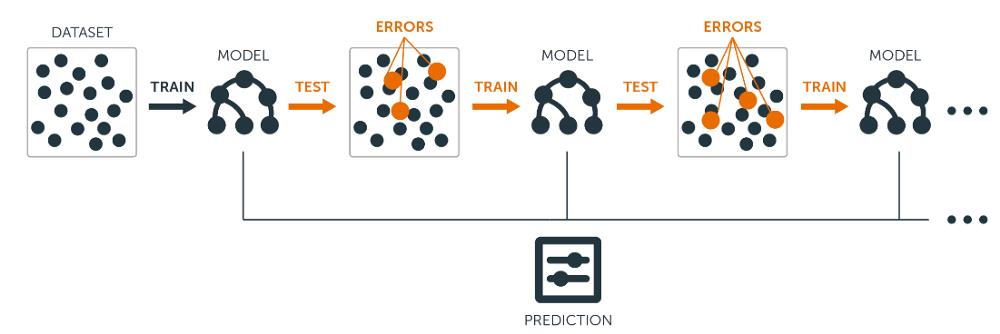
\includegraphics[width=12cm, keepaspectratio]{diagrams/boosting.jpg}
	\center
	\captionof{figure}{Data flow of gradient boosting machine \cite{boostingFigureReference}.}
	\label{fig:Boosting}
\end{center}

Boosting as a ensemble method focus at reducing bias, so the base models are often considered for boosting models with low variance and high level of bias. For comparison to bagging, this approach can not be done in parallel. However, it requires careful tuning of different hyper-parameters.
Boosting involved into powerful forms i.e.: Arcing\cite{ArcingBoosting}, AdaBoosting\cite{AdaBoostBoosting}, Gradient Boosting \cite{GradientBoosting}, XGBoost \cite{XGBoosting}.

\newpage
\section{Multi agent system}

Multi agent system also known as "self organized system" is a computerized system constructed by many agents who interact with each other. Multi-agent systems can solve many complex problems that are a may be insoluble using monolithic systems. 

The system inherits features from active autonomous agents that make up the agent system. A group of agents creates a system and has its own properties such as: autonomy, rationality, activity, goal orientation, adaptability and mobility.

The multi-agent system strives to achieve the set global goal and takes place in a \textit{decentralized} mode. In the consequence of autonomously decisions made by agents, the set goal is achieved. In general, no agent is favored or privileged, and therefore cannot enforce actions on other entities. The ability to \textit{self-organize} (or reorganize), which is done to a certain extent by agents, is the reason for pursuing the set goal. Mechanism of synchronization and coordination of activities in the system is not strictly defined (it is not imposed externally or centrally). Therefore, \textit{asynchrony} is an important feature that describes this type of system.
System under consideration is characterized by \textit{openness} - it means that an agent can join or resign from participation in the pursuit of global goals at any time. There is a need to implement mechanisms to respond by this feature (area of communication and organization). It is worth noting that the \textit{interopability} feature reinforces the property of openness of the agent system. As a result, agents who do not come from this project (they were built up in another production process) may join such a system. New quality is brought by the mobility of agents. Thanks to the system \textit{dispersion}, all operations can be spaced apart in space, which allows easy scaling and load balancing. It is worth noting that the future agent's state is \textit{difficult to predict}. This problem occurs as a consequence of the fact that agents are autonomous entities. In summary, even knowledge of the functioning of autonomous agents does not guarantee full knowledge and ability to predict the effects of interactions in the system.

Widely used approach to system design and evolution necessitated various modifications classic agent system. Many new extensions based on (MAAI) multi-agent systems of artificial intelligence have been proposed, for example: DAI - Distributed Artificial Intelligence System. DAI and other modifications have been already applied for simulating societies, Modelling Social Systems, in the field connected with climate, energy, epidemiology, conflict management and much more. These system designing is highly popular where increasing demands are placed on the amount of data processing (big data), processing time, scaling, high availability and ability to make autonomous decisions.


\subsection{Learning by the agent}

As Russel and Norvig \cite{SLStructure} have designed structure of learning agent architecture to four elements:
\begin{enumerate}
	\item learning element,
	\item performance element,
	\item critic element,
	\item problem generator
\end{enumerate}

\begin{center}
	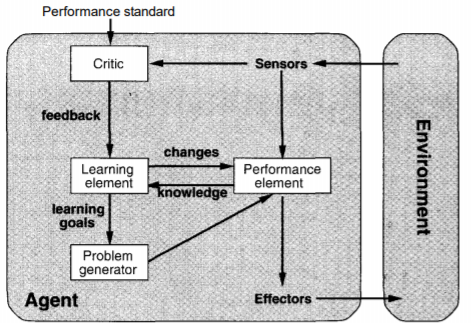
\includegraphics[width=8cm, keepaspectratio]{diagrams/related_work/SLAgents}
	\center
	\captionof{figure}{A general model of learning agents \cite{SLStructure}.} 
	\label{fig:RelatedWorkAgentLearning}
\end{center}

On the figure ~\ref{fig:RelatedWorkAgentLearning} are shown these elements and main interaction patters. Agent perceives on every moment and makes a decision depends on performance input \cite{SLKhaled}. On the one hand the agent uses feedback to determine what should be improved to increase the performance. On the other hand, the problem generator introduce agent to new informative experiences through suggesting actions.

\subsection{Environment}

The appearing 'agent system environment' statement thesis whether the agent system is modelled separately or with it. The answer to the thesis is the approach used to describe the phenomena occurring in the surrounding environment. An object representing the environment in a relatively isolated agent system would perform all these processes inside.
Then there is the necessity to place responsibility contact-agents as a boundary between the system and the environment. However, the environment as non-restrictionized gives environmental field depending on the need for its modelling.


When enriching with the agent system environment model, general formal conditions have been imposed:
\begin{itemize}
	\item the environment of this system is modelled by an isolated system and intentionally specified from the system environment,
	\item the boundary between the agent system and the environment in question is set up using contact agents and their possible external actions,
	\item the environment model created accepts changes in its state as a result of agent's actions and offers the opportunity to observe changes in states using other actions,
	\item if required, the dynamics of the environment is modelled independently. There is a chance to observe the changes taking place in this dynamics.
\end{itemize}

Environmental properties generate many decisions when designing the agent system architecture for a specific application. The general environment's characteristics of this system mainly apply to the functions of agents that they are to fulfil when designing architecture. There are many aspects to consider when defining the broadly understood term "environment in an agent system".

\subsubsection{Observability}

First of all, the observability of the environment by a particular agent affects his ability to take action. An important aspect is also what an agent can observe and which information extracted from the environment is actually needed to take the appropriate action. The following observability scale was adopted due to the level of the agent's perception of the environment:

\begin{itemize}
	\item full observable - when the agent can get full and complete information needed for his action mechanism. The agent operates in the conditions created so-called "full information",
	\item partial observable (partial unobservable) - when the agent does not work in conditions where it has access to full information. Through this type of approach, an agent can make suboptimal, but still practical decision that are crucial for the proper functioning of the agent system,
	\item unobservable - when agent does not have access to the information that he needs to perform the intended action. This agent can complete the necessary knowledge using another agent who has the ability to observe the environment,
	\item relative observability - occurs when the environment is unobservable for all agents and they must derive knowledge through contact agents. Relative property is very often overlooked in the literature.
\end{itemize}

In the presented system only by communication it is possible to solve problems related to the lack of adequate environment's observability. In fact, the terms accessible/inaccessible are used instead of relative observability. However, it has been noted that, among others, through relative observability, agents organize themselves into the system and make suboptimal decisions.

\subsubsection{Stability}

Secondly, general characteristics of the environment also describes the type of environment. Resolving between dynamic and static environments is possible by determining if agent actions are able to change the state of the environment.

The environment is \textit{static} for each agent in this system if these agents do not change the state of the environment. It was stated that the static statement will clearly determine how the environment works (no relative static).

The agent system in which the \textit{dynamic} environment operates places high demands on the designed system. Appropriate precision used during the prediction of the environment evolution is the key to the meet requirement when using a dynamically changing system environment. In the described situation, we are not able to clearly determine whether the agents made optimal decisions.

\subsubsection{Determinism}

If there is no uncertainty associated with the new state of the environment and that the defined action brings a clear and properly describe effect, then from the agent's point of view the environment is \textit{deterministic}.

On the other hand, when the agent's interactions and actions are able to cause an unknown response of the reaction model, then the environment is defined as \textit{non-deterministic}. This is due to the poor precision of predicting response to agent interactions. The consequence of this approach may be that the taken actions will be unfavorable or incorrect for the agent.

\subsubsection{Modelling}

The discussion about whether the environment is modelled as \textit{continuous} or \textit{discrete} corresponds to whether the defined agent perception actions sample the state of the environment. Typically, a discrete agent structure is used (hence discrete modelling of the environment), even if there are problems with the quality and reliability of the mapping.

\subsubsection{Episodicity}

This feature facilitates the design of agent systems. During the episode, the agent performs closely related activities. The steps in the algorithm of conduct are short and there are few (except when learning occurs), then there is no need to hold and analyze information about past episodes.

\newpage
\section{Proposed multi-agent system}

\subsection{Architecture}

When designing the architecture of the agent system, it is important to correctly interpret the set functionality requirements. Formulating the purpose of scientific work did not explicitly set the requirements that the system must meet. An additional challenge is to be able to anticipate additional problems before they occur. Architecture must meet all assumptions in accordance with the definition of agent system with autonomous units. The following is the architecture of the agent system that meets the requirements.


\begin{center}
	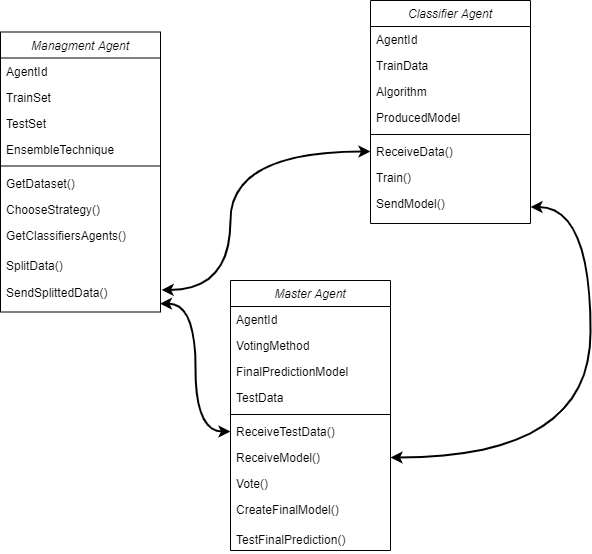
\includegraphics[width=0.70\textwidth, keepaspectratio]{diagrams/architecture-diag}
	\center
	\captionof{figure}{Architecture of proposed agent system.}
	\label{fig:architecture-diagram}
\end{center}



As shown on the figure \ref{fig:MASArchitecture}, system comprises three types of agent: DataManager agent, Classifier agent, Master agent. The proposed agent architecture present data flow and end to end process of creating final prediction model. In presented architecture, each agent has unique objectives and responsibilities. Only working in collaboration, these three types of agents would achieve an overall goal which is accuracy in predicting house price. 


\subsubsection{Communication}

\begin{center}
	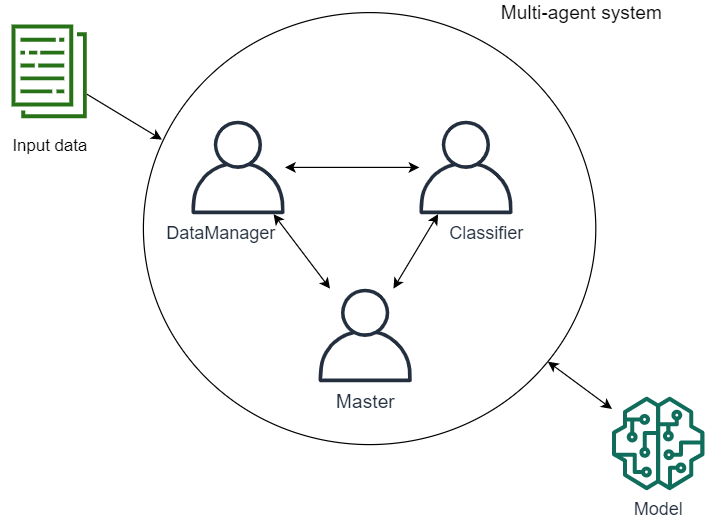
\includegraphics[width=0.65\textwidth, keepaspectratio]{diagrams/architecture}
	\center
	\captionof{figure}{Process of achieving the goal due to communication with 3 classifiers agents.}
	\label{fig:MASArchitecture}
\end{center}


\subsubsection{Environment}

\begin{center}
	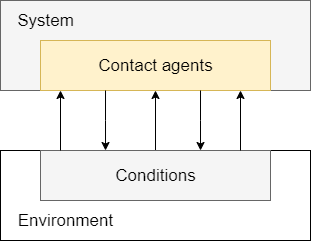
\includegraphics[width=0.35\textwidth, keepaspectratio]{diagrams/env-contact-agents}
	\center
	\captionof{figure}{Architecture of proposed agent system.}
	\label{fig:env-contact-agents}
\end{center}


\subsection{Agents specification}

Presented multi agent system is composed of three main types of agent: management agent, classifier agent, master agent (Fig. 1). Below is presented description of responsibility and interactions for each agent. For every agent of designed system is presented data flow and possible permissions.

\subsubsection{Managment Agent}

The agent receives information (data set) that creates the environment in system. Then he decides which part of the data set to devote to the model's training purposes and which part to extract for testing the obtained prediction. Main responsibility of this autonomous unit is to distribute the training set among classifier agents. 

\begin{center}
	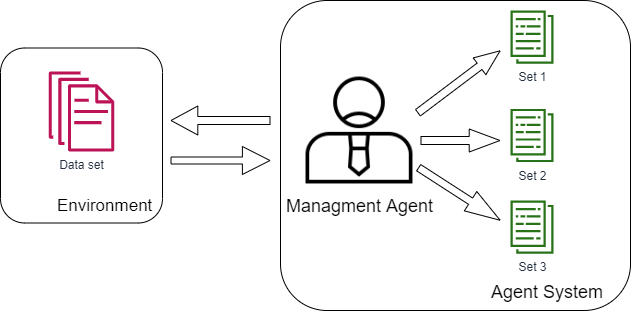
\includegraphics[width=0.65\textwidth, keepaspectratio]{diagrams/managment-agent}
	\center
	\captionof{figure}{Process of achieving the goal due to communication with 3 classifiers agents.}
	\label{fig:ManagmentAgent}
\end{center}

As can be shown on Fig. \ref{fig:ManagmentAgent}, managment agent is a contact agent. It is an interface of other agents to perceive the environment. When choosing a strategy for splitting a data set, the agent decides whether:
 
\begin{itemize}
	\item if each agent receive the same part, 
	\item whether information is to be equally divided for each individual, 
	\item if the agent get full information from a given part (full number of features describing a given observation).
\end{itemize}

\subsubsection{Classifier Agent}

This type of agent is the only one on the system that can occur (and even should) in many cases. In the proposed solution, classifier agent does not have direct access to the environment. Hence, it uses contact agent - management agent that gives him right permissions to perceiving environment. It is treated as a black box in which it receives data on input and a model on output.

\begin{center}
	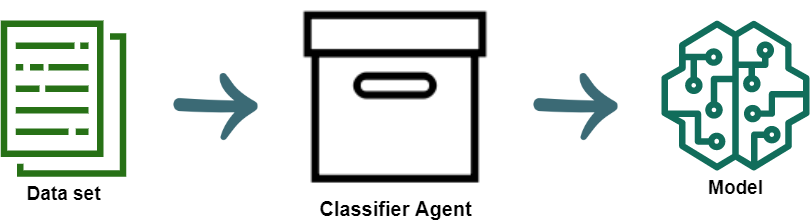
\includegraphics[width=0.55\textwidth, keepaspectratio]{diagrams/black-box}
	%%\center
	\captionof{figure}{Main concept of the classifying agent is the encapsulation machine learning algorithm.}
	\label{fig:ClassifierAgent}
	%%\end{center
\end{center}

As shown on the fig. \ref{fig:ClassifierAgent}, classifier agent does not know if the collection he receives is a complete set. Completeness of the information received says that the agent has get the full number of features for the obtained observations. However, he can only get a certain part of the collection. He does not need to get information from other agents of the same type (who can implement a different type of machine learning algorithm) regarding their perception of the environment. It is planned to perform experiments using following machine learning algorithms: 
\begin{itemize}
	\item K nearest neighbours (KNN), 
	\item Bayesian Ridge, 
	\item Logistic Regression, 
	\item Decision Tree.
\end{itemize} 

Trained model is a result (artifact) of the agent interaction. Then, it communicates with the master agent in order to send him the created model.

\subsubsection{Master Agent}

There is only one instance of this stand-alone agent in the system. Responsibility of this agent is to communicate with classifiers agents in order to receive a trained model from them. Then, he sums up all the trained models to create one final prediction model.

\begin{center}
	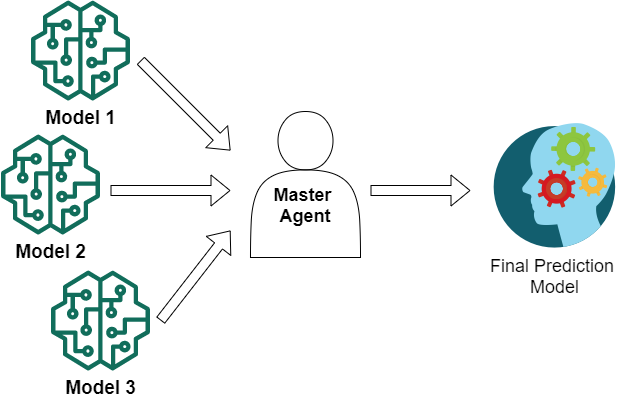
\includegraphics[width=0.65\textwidth, keepaspectratio]{diagrams/master-agent}
	\center
	\captionof{figure}{Process of achieving the goal due to communication with 3 classifiers agents.}
	\label{fig:MasterAgent}
\end{center}

As shown on the Fig. \ref{fig:MasterAgent}, master agent as an autonomous unit is able to sum the received models.
In order for the quality of the received artifact to be as high as possible, master agent can sum the models according to the adopted strategy. So far, several methods have been proposed: 
\begin{itemize}
	\item majority voting - every model instance is important only if receives more than half of the votes. If none of the prediction get more than a half of the votes, it is said that ensemble method might not create a stable prediction for this instance,
	\item weighted voting - modified version of majority voting is done by increasing the importance of one or some models,
	\item simple averaging - every model has same weight and then average model is calculated,
	\item weighted averaging - slightly modified version of simple averaging. Prediction of each model is multiplied by the weight, then average is calculated.
\end{itemize}

Only the \textit{average voting} and \textit{weighted voting} will be examined in experiments. They were chosen because the stated goal of the thesis suggests not to award better quality models. It is not known if a poor-quality predictive model will have a positive effect on the sum with other models.

\section{Summary}
The first section was devoted to a review of the literature related to machine learning issues in agent systems. Quated results and observations were posted that helped to better plan and perform experiments.


Next section focuses on analysing and citing literature where methods of ensemble learning were used. The focus was on three types: stacking, boosting and bagging.

Section contains a theoretical introduction, which has been written based on \cite{Dobrowolski}.The first subchapter related to the general characteristics of agent systems was prepared by the paraphrase of general description in 2nd chapter and "2.6 Characteristics of agent system. Summary" from the cited literature. Theoretical introduction to the definition of the environment in agent system has been completely prepared on paraphrasing subsection "2.2 Agent System as a relatively isolated system".


The last section was devoted to the description of the designed agent system. Aspects such as architecture, environment, communication in the agent system and agent specifications have been described.

%dodac autorów do kazdej publikacji naukowej
%Zastanowić się jak uzyc boosting
%schemat komunikacyjny jako ogolny diagram
%diagram sekwencji (komunikacja głównym agentem a innymi agentami)
%rozna raprezentacja danych (sprawdzic który algorytm lepiej sobie radzi z roznymi typami danych)
%rozdzial toeretyczny wyslac (state of the art)
% uporządkować literaturę zeby była ładnie zrobiona
% przerysować tabele niewyrazne i obrazki jesli sie da
%web risk agent
%https://dl.acm.org/doi/10.1016/j.eswa.2012.01.001

\chapter{Dataset}
\chapter{Background}
% W tym rozdziale przedstawiona jest architektura modeli deep learningowych wykorzystywanych w tej pracy. Najpierw opisane sa podstawowe jednostki z  ktorych skladaja sie sieci neuronowe, a nastepnie wyjasnione sa cale architektury uzytych modeli.
This chapter presents the theoretical background behind the architecture of deep learning models used in this work. First of all the basic units that compose the neural network are described. Then there is an explanation of the whole architecture of the chosen deep learning models.


\section{Neural Network Layers}
% Istnieje duzo typow warstw sieci neuronowych, z ktorych kazdy wykonuje rozne operacje matematyczne, co pozwala mu specjalizowac sie w konkretnych zadaniach. Podczas budowania sieci neuronowej mozna stackowac na sobie rozne warstwy, co pozwala na zbudowanie nieskonczonej liczby roznych modeli. W tym podrozdziale opisane sa wybrane warstwy sieci neuronowych, ktore wykorzystano w tej pracy.
There are many types of neural networks' layers, each of which performs different mathematical operations, which allows it to specialize in specific tasks. When building a neural network, you can stack different layers on each other, which allows you to build an infinite number of different models. This section describes selected layers that were used in this work to build the models .


\subsection{Dense}
Dense layers are super easy pro layers


\subsection{Convolution}
Convolution layers catch local patterns

\subsection{Long-Short Term Memory}
LSTM layers are better than recurrent layers

\subsection{Attention}
Attention layer helps to focus on proper features


\section{Neural Network Architectures}
% Aby dobrze dzialac i skutecznie wykonywac wyspecyfikowane zadanie, model wymaga odpowiednio dobranej architektury. Co roku powstaja kolejne coraz bardziej lub mniej skompikowane schematy wg. ktorych nalezy budowac modele glebokiego uczenia tak aby osiagnac satysfakcjonujace rezultaty. W tym podrozdziale opisane sa schematy architektur sieci neuronowych wykorzystanych w tej pracy.
To successfully perform a specified task, the model requires a properly selected architecture. Every year, more and more complicated schemes are created in order to solve more sophisticated tasks. Usually to obtain satisfactory results, a well known scheme should be followed mhile building a model. This subsection describes the schemes of neural network architectures used in this work.


\subsection{AutoEncoder}
AutoEncoder is unsupervised network.

\subsection{Variational AutoEncoder}
VAE is generative network.

\chapter{Experimental Setup}
\chapter{Results}
\chapter{Conclusions}

\cleardoublepage % to ensure that the page reference is correct
\addcontentsline{toc}{chapter}{\listfigurename}
\listoffigures

\begingroup
	\let \clearpage \relax % to suppress page break

	\cleardoublepage
	\addcontentsline{toc}{chapter}{\listalgorithmname}
	\listofalgorithms
\endgroup

\nocite{*} % forces bibtex to include all citations, whether or not they were referred to in the paper

\cleardoublepage
\addcontentsline{toc}{chapter}{Bibliography}
\bibliographystyle{bib-style}
\bibliography{bibliography}

\end{document}

